\section{Ergebnisse}
In dieser Arbeit wurden 14 unterschiedliche Knochentypen mit je vier verschiedenen Mess-Dimensionen über noch einmal 4 Zeitperioden betrachtet. 
Das sind 14 Diagramme mit je 4 Plots, die an dieser Stelle nicht alle einzeln ausgewertet werden können. 
Ich konzentriere mich daher in der Auswertung auf den Knochentyp »Metatarsal« und hier auf die Dimension »Bp«.
Alle anderen Plots und statistischen Auswertungen finden sich im Ordner \texttt{results}. 

\subsection{Grafische Darstellung der Daten}
Die nun vorbereiteten Daten lassen sich wunderbar in Form sogenannter »Raincloud Plots«\cite{Allen2021} darstellen. Raincloud Plots sind halbe Violin Plots, ergänzt durch einen Scatterplot der Rohdaten und einen Boxplot für eine einfache Übersicht der Mittelwerte und Ausreißer. 
Die Raincloud Plots wurden mit Hilfe des interaktiven Tutorials von \cite{Allen2021} erstellt, zu sehen im \texttt{ab\_plots.ipynb}.

\begin{figure}[H]
    \centering
    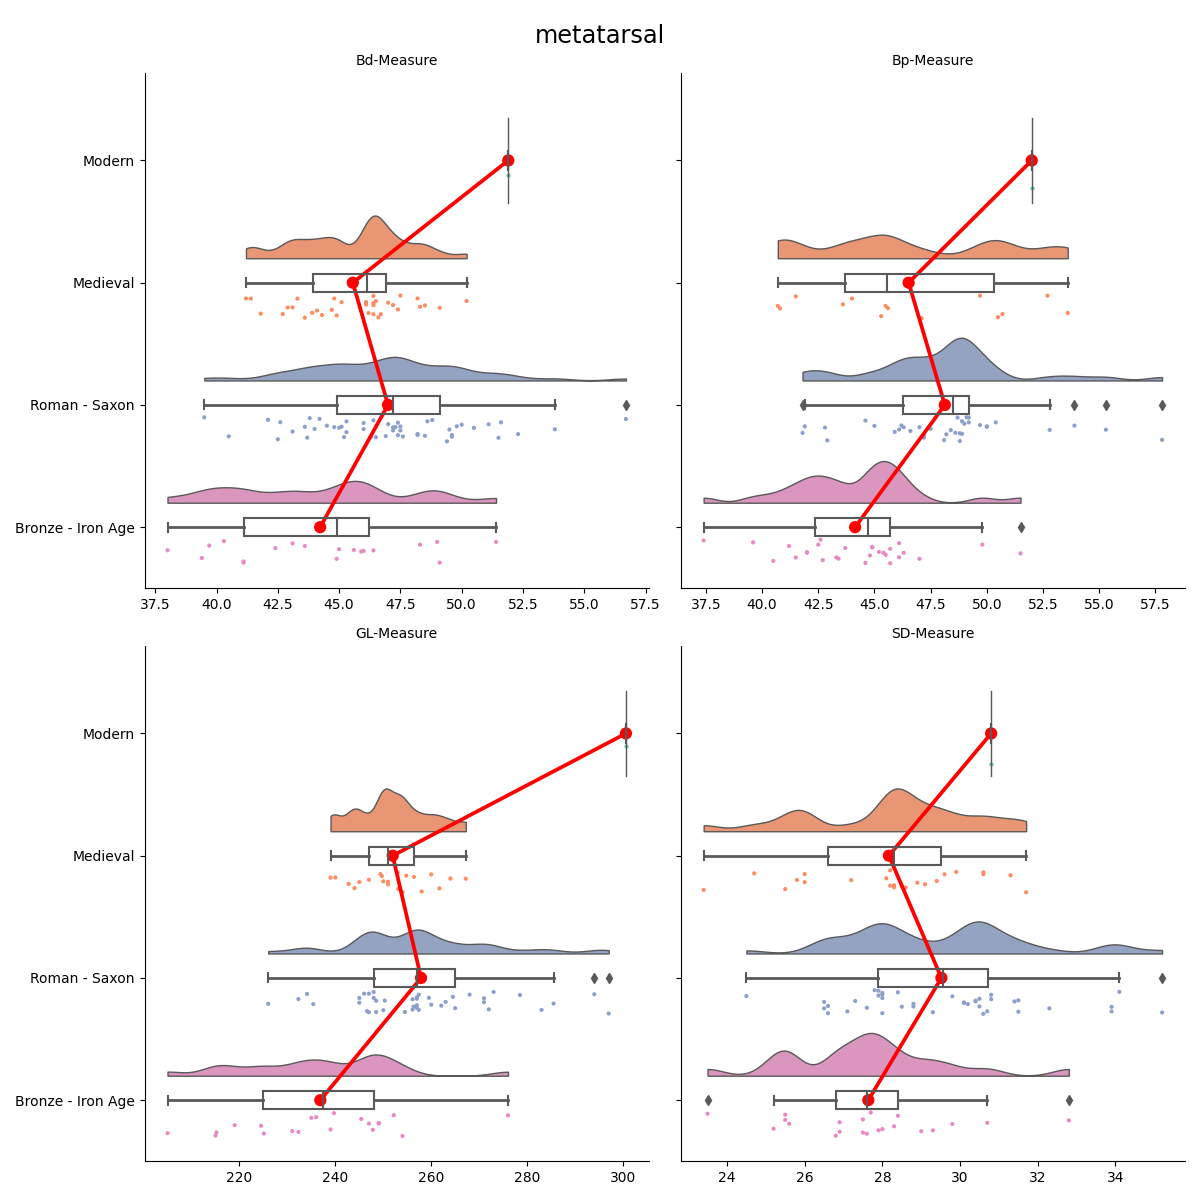
\includegraphics[height=10cm]{plots/rainclouds/metatarsal.png}
    \caption{Raincloud Plots für die Metatarsal Knochen}
    \label{fig:raincloud}
\end{figure}

An \autoref{fig:raincloud} lässt sich gut erkennen, dass die Knochengrößen sich bei allen Dimensionen zwischen den einzelnen Perioden unterscheiden. 
Im Intervall »Roman - Saxon« sind die Knochen in allen vier Dimensionen deutlich größer als sowohl zuvor in der Periode »Bronze - Iron Age« als auch später im »Medieval«. 
Von »Medieval« zu »Modern« nimmt die Größe bei allen vier Dimensionen wieder zu.

\subsection{Statistische Auswertung}
